\section{Лекция 10 - 2023-11-08 - Критерий Вальда}

% TODO начало я пропустил - дописать

% TODO кажется это доказательство всё-таки относиться к прошлой лекции

% \subsection{Критерии отношения правдоподобия}

% \begin{theorem}[Неймана-Пирсона]
%   $\vec{X}_n = (X_1, X_2,\dots, X_n) \sim F(x, \theta)$ тогда критерий уровня $\alpha$ $(S^*, Z(\vec{X}_n)) = \dfrac{\mathcal{L} (\vec{X}_n, \theta_1)}{\mathcal{L}(\vec{X}_n, \theta_0)}$, тогда $\forall 0 < \alpha < 1 \exists \varepsilon \in [0, 1] : \varphi^*(\vec{X}_n) = \begin{cases}
%     1, &z > C \\
%     \varepsilon, &z=C \\
%     0, &z<C
%   \end{cases}
%   $ - является оптимальным среди всех критериев с заданной $\alpha$
  
%   т.е. $\forall$ крит функции $\tilde S$ с $\tilde \varphi$ уровня $\alpha$ $W(S^*, \theta_1) \geqslant W(\tilde S, \theta_1)$ $\Rightarrow$ ошибка $\beta$ меньше.
% \end{theorem}

\begin{ex}[на критерий Неймана-Пирсона]
  $X_1,\dots,X_n \sim N(a, \sigma)$, $a = a_0$ - известно
  $H_0 : \sigma = \sigma_0$
  $H_1 : \sigma = \sigma_1$
  \begin{multline*}
    \dfrac{L(\bar X, \sigma_1)}{L(\bar X, \sigma_0}
    = \prod \dfrac{\dfrac{1}{\sqrt{2\pi} \sigma_1} \exp\left(- \dfrac{(x_k - a_0)^2}{2\sigma_1^2}\right)}{\dfrac{1}{\sqrt{2\pi} \sigma_0} exp\left(- \dfrac{(x_k - a_0)^2}{2\sigma_0^2}\right)}
    = \left(\dfrac{\sigma_0}{\sigma_1}\right)^n exp\left(-\dfrac{1}{2\sigma_1^2} \sum (X_k-a_0)^2 + \dfrac{1}{2\sigma_0^2} \sum (X_k-a_0)^2 \right) = \\
    = \left(\dfrac{\sigma_0}{\sigma_1}\right)^n \exp\left( -\dfrac{1}{2} \sum \dfrac{\sigma_0^2 (X_k-a_0)^2 + \sigma_1^2 (X_k - a_0)^2}{\sigma_1^2 \sigma_0^2} \right) \geqslant C
  \end{multline*}

  \begin{equation*}
    \left(\dfrac{\sigma_0}{\sigma_1}\right)^n \exp\left(-\dfrac{1}{2} \dfrac{\sigma_0^2 - \sigma_1^2}{\sigma_1^2 \sigma_0^2} \sum (X_k-a_0)^2\right) \geqslant C
  \end{equation*}

  На основе знания какая из сигм больше можно уже построить критерий вида:
  $$ S = \left\{ \sum(X_k-a_0)^2 \leqslant (\geqslant) C_1 \right\} $$
\end{ex}

\subsection{Графическая иллюстрация критерия отношения правдоподобия}

\begin{figure}[h!]
  \centering
  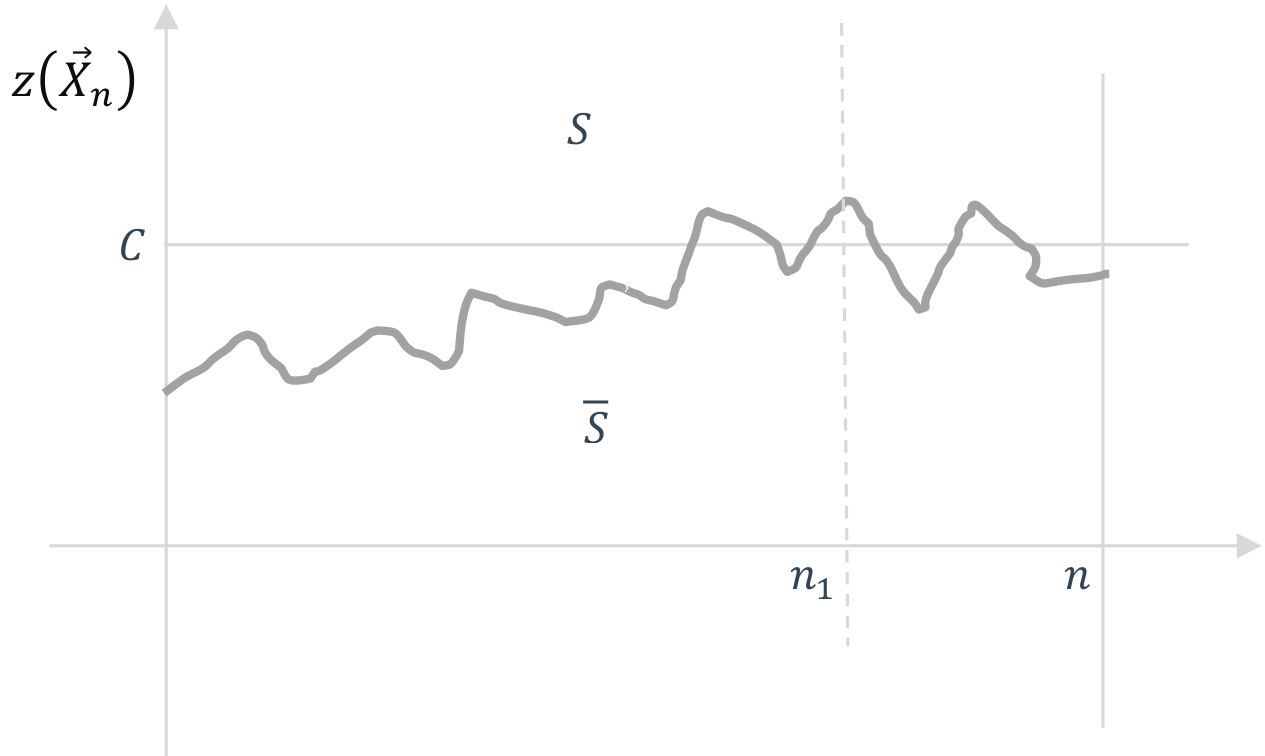
\includegraphics[width=0.8\textwidth]{Figures/10-plot1.png}
  \caption{Иллюстрация критерия Неймана-Пирсона}
  \label{fig:10-plot1}
\end{figure}

Таким образом, вывод по верности гипотез может зависеть от объема выборки n.

\subsection{Графическая иллюстрация критерия Вальда}

\begin{figure}[h!]
  \centering
  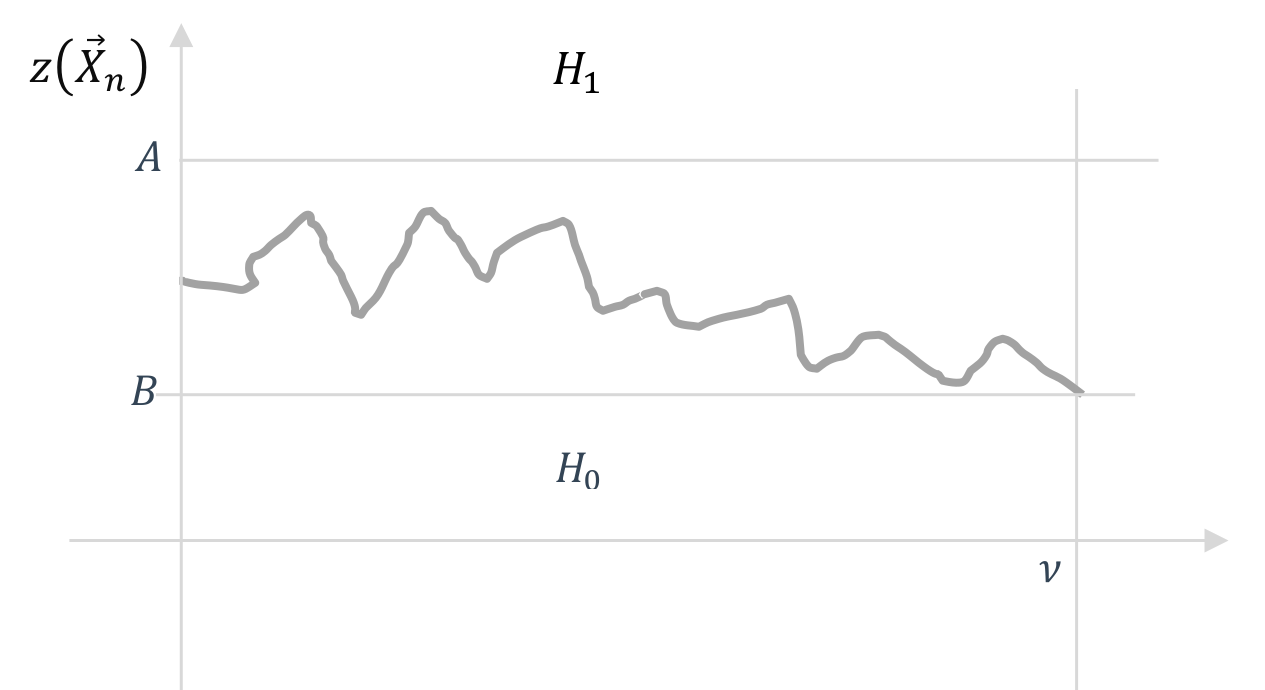
\includegraphics[width=0.8\textwidth]{Figures/10-plot2.png}
  \caption{Иллюстрация критерия Вальда}
  \label{fig:10-plot2}
\end{figure}

На рисунке \ref{fig:10-plot2}:
cнизу область принятия $H_0$;
сверху область принятия $H_1$;
посередине область продолжения наблюдений.
Как только после очередного наблюдения статистика перешла вниз или вверх, наблюдения прекращаются и принимается нужная гипотеза.

Статистика критерия $(\nu, X_1, X_2, \dots, X_n)$,
$\nu = min \{ n : Z_n \notin (B, A) \}$,
$z_n = \dfrac{L(X_1, \dots, X_n, \theta_1)}{L(X_1, \dots, X_n, \theta_0)}$

Критерий: Пусть 0<B<1<A.
$z_\nu \geqslant A$ - принимаем $H_1$; $z_\nu \leqslant B$ - принимаем $H_0$.

\begin{theorem}
  При $i \in \{ 0, 1 \}$:
  \[
    P_{\theta_i}(\nu < \infty) = 1, \exists M_{\theta_0} \nu < \infty, M_{\theta_1} \nu < \infty
  \]
  Здесь $P_{\theta_i} (A)$ обозначена условная вероятность $P(A | \theta_i)$
\end{theorem}

\begin{proof}
  Назовем $Y_k = \ln \dfrac{P(X_k, \theta_1)}{P(X_k, \theta_0)}$, тогда:
  \[
    \ln Z_n = \sum_{k=1}^n \ln \dfrac{P(X_k, \theta_1)}{P(X_k, \theta_0)} = \sum_{k=1}^n Y_k
  \]

  Зададим $r \in \mathbb{N}$, и обозначим:
  \begin{align*}
    \eta_1 &= Y_1 + Y_2 + \dots + Y_r \\
    \eta_2 &= Y_{r+1} + Y_{r+2} + \dots + Y_{2r} \\
           &\dots \\
    \eta_k &= Y_{(k-1) r + 1} + \dots + Y_{kr}
  \end{align*}

  Тогда событие $(\nu > rk)$ означает, что $(\ln B < Y_1 + \dots + Y_j < \ln A, j \leqslant rk)$, а следовательно и $(\ln B < \eta_1 + \eta_2 + \dots + \eta_j < \ln A, j \leqslant k)$.

  \begin{multline*}
    P_{\theta_i} (\nu > kr)
    = P_{\theta_i} (\ln B < Y_1 + \dots + Y_j < \ln A, j \leqslant kr) \leqslant \\
    \leqslant P_{\theta_i} (\ln B < \eta_1 + \eta_2 + \dots + \eta_i < \ln A, j \leqslant k) \leqslant \\
    \leqslant P_{\theta_i} (|\eta_j| < \ln A - \ln B, j \leqslant k)
    = P_{\theta_i} \left(\bigcap (|\eta_j| < \ln A - \ln B)\right) =
  \end{multline*}
  т.к. $\eta_i$ - назависимы и одинаково распределены \\
  \[
    = (P_{\theta_i} (|\eta_i| < \ln (A/B)))^k
  \]

  Выбираем r так, чтобы дисперсия $\eta_1$ была достаточно большой:
  \[
    \forall i : M_{\theta_i} \eta_1^2 \geqslant D_{\theta_i} \eta_1
    = r \cdot D_{\theta_i} Y_j > C^2 = (\ln (A/B))^2,
  \]
  Тогда
  \[
    P(\theta_i) = P_{\theta_i} (|\eta_1| < C) < 1
  \]

  иначе $P_{\theta_i} (|\eta_i| < C) = 1 \Rightarrow M \eta_i^2 < C^2$

  В силу независимости $\eta_j$:
  \[
    P_{\theta_i} (\nu > rk) \leqslant (P(\theta_i))^k = (P(\theta_i)^{1/r})^{rk}
  \]

  Тогда, очевидно:
  \[
    P_{\theta_i} (\nu > rk) \to 0, k \to \infty
  \]
  % TODO не знаю что следующая строчка вообще означает:
  $M_{\theta_i} \nu = \sum n P_{\theta_i} (\nu  = n) = \sum P_{\theta_i} (\nu \geqslant n) = \sum ( P(\theta_i)^{1/r} )^{nr}$
\end{proof}

Вторая особенность такого критерия состоит в том, что он чувствителен к порядку учета выборки.

\begin{theorem}[Вальда]
  Если заданы A и B, то ошибки $\alpha$ и $\beta$ удовлетворяют неравенствам:
  \begin{equation*}
    \begin{cases}
      \dfrac{1 - \beta}{\alpha} \geqslant A \\[1em]
      \dfrac{\beta}{1 - \alpha} \leqslant B
    \end{cases}
  \end{equation*}
  (максимально широкий коридор)

  Эти неравенства называют тождестами Вальда.

  % TODO здесь еще рисуночек (в лекциях на странице 12)
\end{theorem}

Применение: если $\alpha$ и $\beta$ заданы, то берут $A = \dfrac{1-\beta}{\alpha}, B = \dfrac{\beta}{1 - \alpha}$
% TODO расписать в применении, почему берем именно крайние точки из неравенств
Почему так? - иначе сумма ошибок будет больше

\begin{proof}
  $\varkappa_{0n} = \left( \vec{X}_n : B < Z_k < A, k = \overline{1, n-1}, z_n \leqslant B \right)$ - множество тех, которые ведут к принятию гипотезы $H_0$

  $\varkappa_{1n} = \left( \vec{X}_n : B < Z_k < A, k = \overline{1, n-1}, z_n \geqslant A \right)$ - множество тех, которые ведут к принятию гипотезы $H_1$

  \begin{equation*}
    1 = \sum  P_{\theta_i} (\nu = n) = \sum P_{\theta_i} (\varkappa_{0n}) + \sum P_{\theta_i} (\varkappa_{1n}) =
    \begin{cases}
      (1 - \alpha) + \alpha, &\theta_0 \\
      \beta + (1 - \beta), &\theta_1
    \end{cases} 
  \end{equation*}

  \[
    \alpha = \sum P_{\theta_0} (\varkappa_{1n}) \leqslant \dfrac{1}{A} \sum P_{\theta_1} (\varkappa_{1n}) = \dfrac{1 - \beta}{A}
  \]
  
  Рассмотрим почему среднее неравенство верно. Для дискретного случая:
  \[
    P_{\theta_1} (\varkappa_{0n}) = \sum_{\vec{X_n} \in \varkappa_{1n}} P_{\theta_1}(\xi_1 = X_1, \dots, \xi_n = X_n)= \sum \mathcal{L} (X_1, \dots, X_n, \theta_1) \leqslant \dfrac{1}{A} \sum \mathcal{L} (\dots, \theta_1) = \dfrac{1 - \beta}{A}
  \]

  \[
    \beta = \sum P_{\theta_1} (\varkappa_{0n}) = \sum_{n=1}^\infty \sum_{\vec{X}_n \in \varkappa_{0n}} P_{\theta_1} (\vec{\xi} = \vec{X}_n)
  \]
\end{proof}

\subsection{Среднее число испытаний в критерии Вальда}

Критерий Вальда для выборки $X_1, \dots, X_n, \dots$.
Рассматривается статистика
\[
  z_n = \dfrac{\mathcal{L} (X_1, \dots, X_n, \theta_1)}{\mathcal{L} (X_1, \dots, X_n, \theta_0)}
\]
если она выходит из коридора $(B, A)$, прекращаем наблюдения и делаем вывод о верности
гипотез.

Обозначим за $\nu$ - номер испытания (или размер выборки, что то же самое),
на котором закончили наблюдения.

\[
  Y_k = \ln \dfrac{P(X_k, \theta_1)}{P(X_k, \theta_0)}
\]

Критерий $z_\nu = \sum \ln \dfrac{P(X_k, \theta_1)}{P(X_k, \theta_0)} = \sum Y_k$
\[
  \nu = \min \{ k, z_k \notin (B, A)\}
\]
Сам критерий Вальда тогда:
\begin{align*}
  z_\nu &\geqslant \ln A \Rightarrow H_1, \\
  z_\nu &\leqslant \ln B \Rightarrow H_0
\end{align*}


Таблица вероятностей ошибок:
\begin{center}
\begin{tabular}{|c|c|c|}
  \hline
  z_\nu & \approx \ln A & \approx \ln B \\
  \hline
  H_0 & \alpha & 1 - \alpha \\
  \hline
  H_1 & 1 - \beta & \beta \\
  \hline
\end{tabular}
\end{center}

Найдем матожидание числа испытаний
\begin{align*}
  M_0 \nu &= \dfrac{M_0 z_\nu}{M_0 Y_k} = \dfrac{\alpha \ln A + (1-\alpha) \ln B}{M_0 Y_k} \\
  M_1 \nu &= \dfrac{M_1 z_\nu}{M_1 Y_k} = \dfrac{(1-\beta) \ln A + \beta \ln B}{M_1 Y_k}
\end{align*}
где $M_0 Y_k$, $M_1 Y_k$ вычисляется уже в конкретном примере из законов распределения.

\begin{proof}
  В соответствии с нашими обозначениями:
  \[
    z_\nu = \sum Y_k \Rightarrow M_i z_\nu = M_i \nu M_i Y_k, i = 0, 1
  \]
  \epigraph{не просто, а очень просто}{Т.~В.~Облакова}
\end{proof}
